\section{Advancements in Digitizer-enabled Neutron \tot\ Measurements of Rare
Isotopes}
By applying newly-available digitizer technology to reduce per-event deadtime,
we have advanced a program of isotopic \tot\ 
measurements valuable for constraining the isovector strength of the nuclear potential at positive 
energies. New data have been obtained on \oEight, \niEightFour, \snTwelveFour\ up
to 450 \mega\electronvolt, dramatically expanding the coverage of these nuclei
and laying the groundwork for subsequent optical model analyses. At the same
time, we have identified shortcomings in the digital-signal-processing approach
that must be rectified in future measurements, namely, the uncertainty in the
true analytic deadtime and in the deadtime associated with digitizer buffer
readout to the data acquisition computer. These effects depend on
the proprietary digitizer firmware algorithms used for peak
identification and buffer management, both of which are opaque to the
end user. In an ideal experiment, DPP and raw waveform traces should be collected
in parallel throughout the experiment and compared during data analysis to
pinpoint any weaknesses in the peak-detection algorithm and identify variations in the analytic
deadtime. Due to the ferocious data rate, we could only
collect small snippets of raw waveform data, insufficient for a full
DPP-raw-waveform comparison.
To resolve the discrepancy in our results above 100
\mega\electronvolt\ with those of \cite{Finlay1993} and \cite{Abfalterer2001},
we suggest two types of benchmarking experiments in the future. First is a
two-digitizer experiment: the same detector signals are fed into two
separate time-synchronized digitizers, one running only in DPP mode,
and one running in raw waveform mode. During analysis, a simulated DPP-mode peak sensing
algorithm can be developed, applied to the real raw waveform-mode data, and its
results compared with the real DPP-mode data, clarifying the DPP-mode behavior of
the digitizer firmware. The second experimental setup would use
both a digitizer and analog electronics:
the same signals would be fed both into the digitizer, as
in our experiment, and into analog-electronics logic utilizing a ``looking
period'' (shown in Fig. \ref{AnalogLogic}).

\section{Implications of DOM Results}
Our DOM analyses of \oSixEight, \caAughtEight, \niEightFour, \snTwelveFour,
and \pbEight\ have yielded new insight into the validity of the DOM approach
and what experimental data are most needed for improved calculations of
essential structural quantities. Our successful fits of \oSixEight\ show that
even lighter systems (e.g., \cTwelve) may be amenable to a non-local DOM
treatment, providing a bridge between ab initio calculations and
phenomenological optical models. The shape of the imaginary potential
above the Fermi energy is consistent across all our fits and agrees
qualitatively with the state-of-the-art global optical model of \cite{KoningDelaroche}. 
Below the Fermi energy where experimental data are much sparser, we see
significant variation in the shape of the potential between nuclei especially
near the Fermi surface, where the magnitude of the imaginary potential changes
rapidly. This is most conspicuous in the lighter nuclei where a reduced level density
makes a smooth optical potential a poor approximation.
Heavy nuclei have sufficient phase space and level density on both
sides of the Fermi energy that the nuclear potential is largely symmetric near
the Fermi energy, in keeping with the expectations of Mahaux and Sartor \cite{Mahaux1991}.

\begin{table}[tb]
    \begin{minipage}{\textwidth}
        \caption[Sensitivity of optical potential terms to the experimental nucleon
        scattering data types]
        {
            Sensitivity of optical potential terms to the experimental nucleon
            scattering data types used in our fit. The typical range of
            available experimental data roughly corresponds to that used for our
            DOM treatments. Parameter terms are detailed in Section
            \ref{PotentialParameterization}.
        }
        \label{ParametersPositiveEnergy}
        \centering
        \begin{tabular}{G N M N M}
            \toprule
            \multirow{2}{*}{Data type} & \multicolumn{2}{c}{Protons} &
            \multicolumn{2}{c}{Neutrons}\\
            \cmidrule(l{0.5em}r{0.5em}){2-3}
            \cmidrule(l{0.5em}r{0.5em}){4-5}
            & Typ. range [\mega\electronvolt] &
            Affected terms & Typ. range [\mega\electronvolt] &
            Affected terms\\
            \midrule
            \el &  $0-200$ & $V_{vol}$, $V_{so}$ & $0-100$ & $V_{vol}$, $V_{so}$\\
            \addlinespace[1.0em]
            AP* &  $0-200$ & $V_{vol}$, $V_{so}$ & $0-100$ & $V_{vol}$, $V_{so}$\\
            \addlinespace[0.5em]
            \rxn & $0-100$ & $W_{sur}^{+}$, $W_{vol}^{+}$, $W_{NM}^{+}$ & $14.1$ &
            $W_{sur}^{+}$\\ 
            \tot & -- & -- & $0-100$ & $V_{vol}$, $V_{so}$, $W_{sur}^{+}$,
            $W_{vol}^{+}$, $W_{NM}^{+}$\\
            \bottomrule
            \multicolumn{2}{l}{\footnotesize*Analyzing Power}
        \end{tabular}
    \end{minipage}
\end{table}
\begin{table}[tb]
    \begin{minipage}{\textwidth}
        \caption[Sensitivity of optical potential terms to bound-state
            experimental data types]
        {
            Sensitivity of optical potential terms to the bound-state 
            experimental data types used in our fit. The typical range listed
            here refers to the choice of incident particle momentum used to perform the
            measurement. Parameter terms are detailed in Section
            \ref{PotentialParameterization}.
        }
        \label{ParametersNegativeEnergy}
        \centering
        \begin{tabular}{c N M}
            \toprule
            Data type & Typical range & Affected terms\\
            \midrule
            (e,e) & \makecell{q-range:\\$0.5-3.5$ \per\femto\meter} & $V_{vol}$, $V_{asym}$,
            $W_{vol}^{\pm}$, $W_{NM}^{-}$\\
            \addlinespace[0.5em]
            (e,e'p) & \makecell{p-range:\\$70-200\ \mega\electronvolt/\text{c}$ } & $W_{sur}^{-}$, $W_{vol}^{-}$\\
            \addlinespace[0.5em]
            $\langle r^{2} \rangle ^{\frac{1}{2}}$ & -- & $V_{vol}$, $W_{sur}^{-}$\\
            \addlinespace[0.7em]
            SP Levels & -- & $V_{vol}$, $V_{so}$\\
            \addlinespace[0.5em]
            Binding Energies & -- & $V_{vol}$, $W_{vol}^{-}$, $W_{NM}^{-}$\\
            \bottomrule
        \end{tabular}
    \end{minipage}
\end{table}

Tables \ref{ParametersPositiveEnergy} and \ref{ParametersNegativeEnergy}
summarize our understanding of the
sensitivity of optical potential terms to the many experimental data types
used in our fit. As discussed in Chapter \ref{introduction} and shown in
Appendix \ref{DOMDataSets}, there is an abundance of nucleon elastic scattering data
from 0-200 \mega\electronvolt\ on many isotopic targets. Equipped with these data, optical-model 
analyses have tightly constrained the magnitude and shape of the \textit{real}
components of the self-energy (in our treatment, the central potential
and spin-orbit components). Unsurprisingly, the gaps in our knowledge of the self-energy are
largest for \textit{imaginary} terms, especially in areas where experimental
data are sparsest.
In our parameterization, this meant that the imaginary potential
above 100 \mega\electronvolt\ ($W_{vol}^{+}$) and at all
energies below the Fermi surface ($W_{vol}^{-}$) were difficult to constrain due
to lack of data. At small positive energies, the imaginary strength
$W_{sur}^{\pm}$ was relatively well-constrained by the handful of proton
\rxn\ studies from 20-80 MeV all more than a decade old \cite{Carlson75,
Slaus1975, Ingemarsson1999, Auce05}. These crucial mid-energy
proton \rxn\ data streamlined the fitting
process for \oSix, \caAughtEight, \niEight, and \pbEight\ and added confidence
in the quality of our fits.
Unfortunately, proton \rxn\ data between 100-200 MeV were available
only for \caForty\ and \pbEight, so a chart-wide study of the evolution
of the proton imaginary strength remains out of reach. To understand the
asymmetry-dependence of the imaginary strength from 100-200 MeV, our new \tot\
results only contribute to the neutron half of the story. New proton \rxn\
measurements above 100 MeV would provide the other.

In preliminary fits that did not include the binding energy,
we found that the deep negative imaginary strength, essentially $W_{vol}^{-}$,
was very poorly constrained. These early fits gave far too small a binding energy,
roughly 2-4 $\mega\electronvolt/\text{A}$.
The inclusion of the binding energy as a fitting constraint
had a dramatic impact on the imaginary terms in the potential: not only did
$W_{vol}^{-}$ grow considerably,
but the imaginary non-locality $\bm{\beta_{4}}$ grew from $\approx$
0.6 \femto\meter\ to $\approx$ 0.9 \femto\meter, affecting the
angular-momentum-dependence of the imaginary strength at all energies.
With the binding energy included, all our fits indicate that a significant
fraction, as much as half, of the nuclear binding energy is generated by a small
fraction of the total nucleon density at very negative energies ($<$-50 \mega\electronvolt).
To understand why, a comparison to mean-field models is useful.
In real nuclei near the Fermi surface, there is
little absorptive strength and thus the spectral functions for nucleons are
primarily discrete peaks. In this regime,
mean-field models can give an excellent description of nuclear behavior as the
assumption of independent particle motion (and a discrete spectrum) is appropriate.
However, at very negative energies with larger imaginary strength,
spectral peak broadening is dramatic and adds a small, but significant,
single-particle occupation at very negative energies, occupation
that plays an outsized role in binding. If our interpretation is
correct, it would partially explain the underbinding of
nuclei in shell models as a failure to account for spectral peak broadening
beyond the valence space of the model. While our optimized fits produced a
binding energy per nucleon roughly 2 $\mega\electronvolt/\text{A}$ below the experimental
values, our results indicate that the binding energy is quite useful for
constraining the imaginary potential strength at negative
energies.

By comparison to experimentally-measured charge density distributions, we see 
that significant depletion of s-shell occupation is needed to reproduce the
proton density in the nuclear core. This depletion should occur in all bound
shells as a consequent of short-range and long-range correlations and
significantly alters the proton and neutron matter distributions.
It is clear in our analysis that the matter distributions are sensitive
to the proton and neutron single-particle configurations as anticipated by
Wilkinson \cite{Wilkinson1967} and Myers \cite{Myers1969} several decades ago.
To wit, the neutron skin thickness we
extract for \oEight\ (0.197 \femto\meter) appears
to be as large or larger than that of
\pbEight\ (0.200 \femto\meter), even though the asymmetry ratio of \pbEight\
(0.212) is almost twice as large as that of \oEight\ (0.111). In light of this
result, we expect that the neutron skins may balloon in $^{52}$Ar and $^{54}$Ca
with the filling of the $\nu$ \fSeven\ and \fFive\ subshells, but grow more slowly
in even heavier Ar and Ca isotopes. Future experiments at FRIB and other
radioactive beam facilities will probe this region and clarify the relative
importance of the asymmetry ratio and high-spin intruder subshells in determining
the neutron distribution near the dripline.

\begin{wrapfigure}[11]{i}{0.5\textwidth}
    \centering
    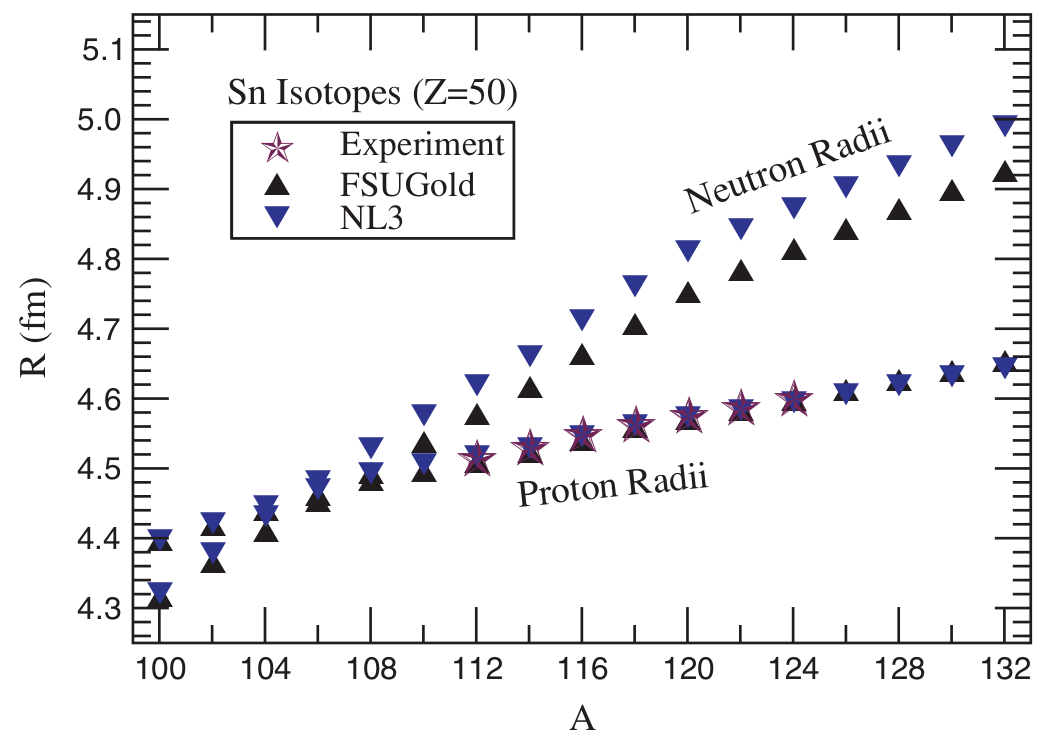
\includegraphics[width=0.48\textwidth]{figures/Piekarewicz2006SnIsotopes.png}
    \caption[Proton and neutron RMS radii in the Sn isotopes computed with FSUGold and NL3
    interactions]
    {
        Proton and neutron RMS radii in the Sn isotopes computed in a relativistic mean-field
        approximation using the FSUGold and NL3 parameter sets, with experimental data for comparison.
        Figure and caption used with permission from \cite{Piekarewicz2006}.
    }
    \label{Piekarewicz2006SnIsotopes}
\end{wrapfigure}
In relativistic and non-relativistic mean-
field models, the neutron skin,
electric dipole
polarizability, and dipole resonances of neutron-rich nuclei are
shown to be tightly correlated with the density-dependence of the symmetry
energy, $L$.
\begin{figure}[tb]
    \centering
    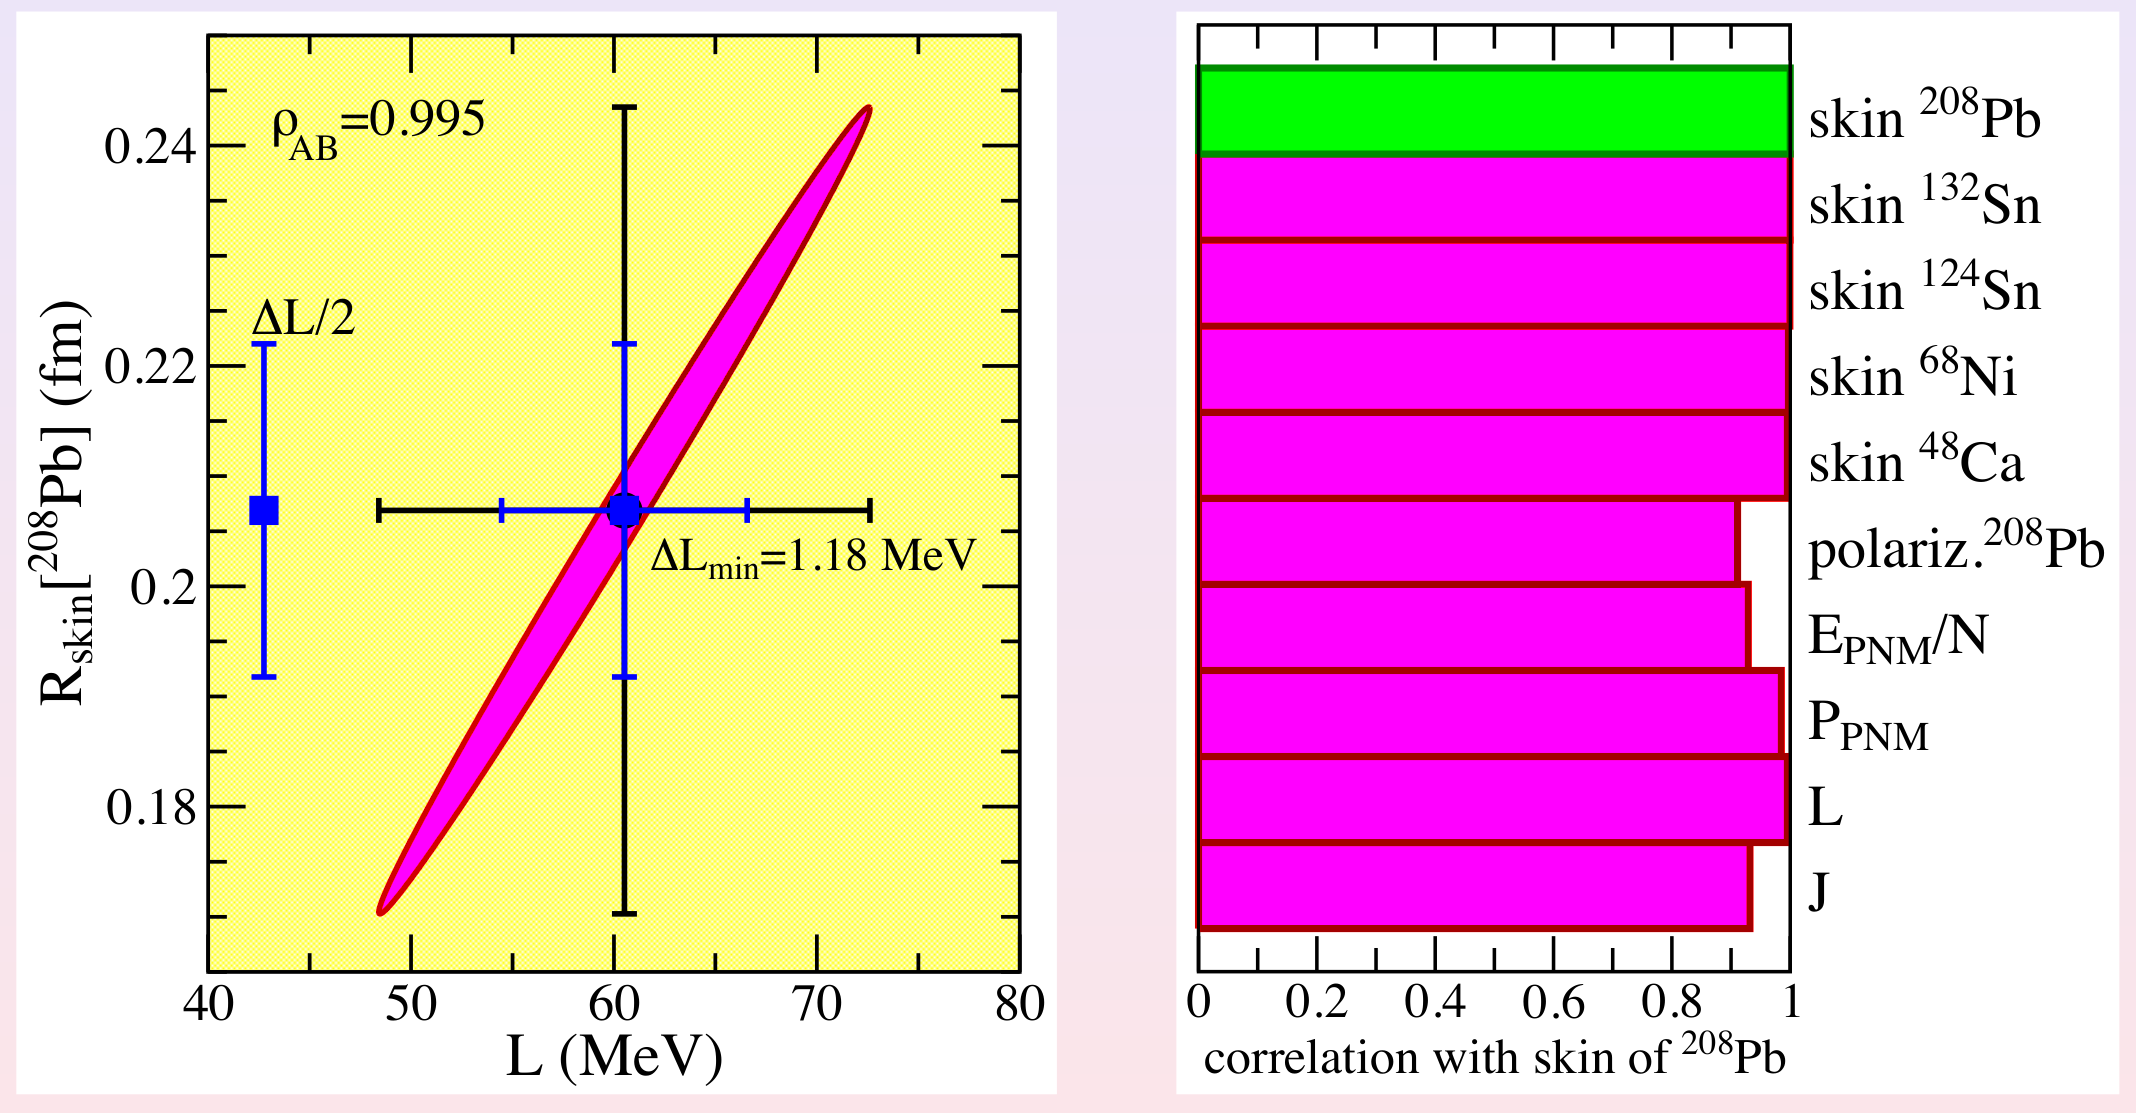
\includegraphics[width=0.9\textwidth]{figures/PiekarewiczPb208SkinCorrelation.png}
    \caption[Correlation between the neutron skin of \pbEight\ and several nuclear structure
    observables]
    {
        Correlation between the neutron skin of \pbEight\ and several nuclear structure observables,
        per a relativistic mean-field calculation with the FSUGold interaction
        conducted by J. Piekarewicz. Many
        mean-field models recover a very strong correlation between the size of the
        neutron skin of several neutron rich nuclides and the density-dependence of the symmetry
        energy, $L$. Figure used with permission.
    }
    \label{PiekarewiczPb208SkinCorrelation}
\end{figure}
While some of our neutron skin predictions are in agreement with those extracted
from state-of-the-art mean-field models, the
full story is not at all clear.
As an example, Fig. \ref{PiekarewiczPb208SkinCorrelation}
shows the results of a covariance analysis on a variety of nuclear structure
quantities as calculated by a relativistic mean-field model 
that employs an FSUGold interaction \cite{Fattoyev2012}.
The neutron
skin for \pbEight\ generated by our fit is in good agreement with this model.
However, another treatment that uses the same interaction
\cite{Piekarewicz2006} gives a neutron skin for \snTwelve\ of roughly 0.09
\femto\meter\ (see Fig. \ref{Piekarewicz2006SnIsotopes}), much \textit{larger} than the
-0.01 \femto\meter\ predicted by our fit.
Understanding the model-dependence of these predictions, both from relativistic mean-field
approaches and from the DOM, is critical for making progress on constraining
$L$. As has been pointed out by other authors, a multi-pronged approach 
is warranted and should include electroweak measurements like PREX \cite{Horowitz2014}, comparison of
charge radii in mirror nuclei \cite{Brown2017}, modeling of dipole
polarizability \cite{Piekarewicz2006}, and multi-messenger astrophysical
measurements on neutron stars. With the expanded scope of the DOM introduced in
this work, we hope to add our new predictions to the mix.

Last, a few comments should be made about the DOM parameterization choices made
in this work. While we have found that the neutron
skin is inflated with the filling of the high-angular-momentum neutron subshells, we
have also seen significant variation in the skin thickness depending on small
changes in the parameter values. In the present treatment, to reduce the risk
of overfitting, we reduced
the total number of parameters to 34, less than half as many as used in
other DOM analyses by our group. As a consequence, it appears that we have
discarded some important physics: we were unable to recover, for example, the full
binding energies and the experimentally-known RMS charge radii for most of the
isotopes we analyzed. Further, the momentum distributions we generate for protons and
neutrons likely underestimate the amount of high-momentum content, especially
for protons in neutron-rich systems. As mentioned earlier, the absence (and
value) of high-energy proton \rxn\ plays an important role in resolving these
discrepancies. A comprehensive error analysis is required
to identify which parameters, if any, should be reintroduced to accommodate
missing physics while keeping the total number of parameters to a minimum.

\section{Additional Directions for Future Study}
In light of the advances and limitations of this work, we identify several
additional avenues of research worth pursuing.
Besides the digitizer benchmarking experiments described earlier
in this chapter, \tot\ measurements on the stable Fe and Cd isotopes would
supplement our Ni and Sn isotope studies and provide much-needed information
about optical-potential isovector dependence outside closed proton shells.
Data for \tot\ on the intermediate stable isotopes $^{114,116,118,120,122}$Sn
would improve optical-model extrapolations to $^{100}$Sn and $^{132}$Sn,
both of which are valuable for testing shell-model validity near the driplines.
We reiterate the importance of new proton \rxn\
studies across the chart of nuclides, particularly on closed-shell isotope and isotone
chains.

A major defect in the DOM treatment presented here is
the lack of covariance analysis of DOM parameters. Without theoretical error
bars associated both with uncertainty in the experimental data used and in the
DOM's parameteric forms, comparisons between the DOM and other models cannot be
complete. Such an analysis would also help reveal exactly which experimental
data are most needed to clarify the murkier energy domains in our fits (e.g.,
the imaginary potential below -100 \mega\electronvolt\ and above 100
\mega\electronvolt). A first step toward this goal is publication of the DOM codebase, a
priority of our group. Even in the absence of appropriate error analysis, 
the single-particle densities and overlap functions generated by DOM fits can be
immediately applied for calculations of coherent neutrino scattering \cite{Herraiz2009} and
scattering of potential dark matter candidates on common detector materials \cite{Anand2014}.

We close by noting that without a wide variety of fundamental experimental nuclear data on stable
targets -- at high and low energies, both for elastic and inelastic scattering,
and probing both protons and neutrons -- systematic analyses like that of the DOM are not possible.
Even as radioactive beam facilities reach further toward the driplines, the capacity for basic 
scattering experiments on stable targets is vital for illuminating the relationship between nuclear 
structure and reactions.
